The energy deposited in the calorimeter cell is proportional to the
reconstructed amplitude. The amplitude is originally measured in ADC counts and
needs to be converted in GeV for physics analysis using the formula:
\begin{equation}
  \label{eq:84}
  E[GeV] = \hat{A}[ADC] \times C_{ADC \rightarrow pC} \times C_{\text{laser}}
  \times C_{Cs} \times C_{pC \rightarrow GeV}
\end{equation}
where $\hat{A}[ADC]$ is the amplitude estimate in ADC counts, $C_{ADC \rightarrow
pC}$ is determined using the \gls{cis}, $C_{pC \rightarrow
  GeV}$ is measured during testbeam using electrons with a well defined energy
and converts the deposited charge to energy in GeV, the laser system allows to
determine the value of the $C_{\text{laser}}$ constant while the Cesium sets the
$C_{Cs}$ factor.

The CIS calibrates the read out electronics by injecting a known charge and
measuring the resulting response of the electronics. The \emph{laser} system
main purpose is to monitor the photomultipliers tubes stability and the
downstream electronics. Well calibrated light pulses are sent to the PMTs and by
reconstructing the signal it is possible to extract the PMTs' gain. The
\emph{cesium} system, circulates a Cs source through each scintillating tile
using an hydraulic system, the PMTs signal is continuously read out through an
integrator. The cesium system allows to equalize the calorimeter cell response
to that measured during test beams. Figure~\ref{fig:cali_chain} depicts a
schematic representation of the ATLAS TileCal calibration chain.

\begin{figure}[!h]
  \centering
    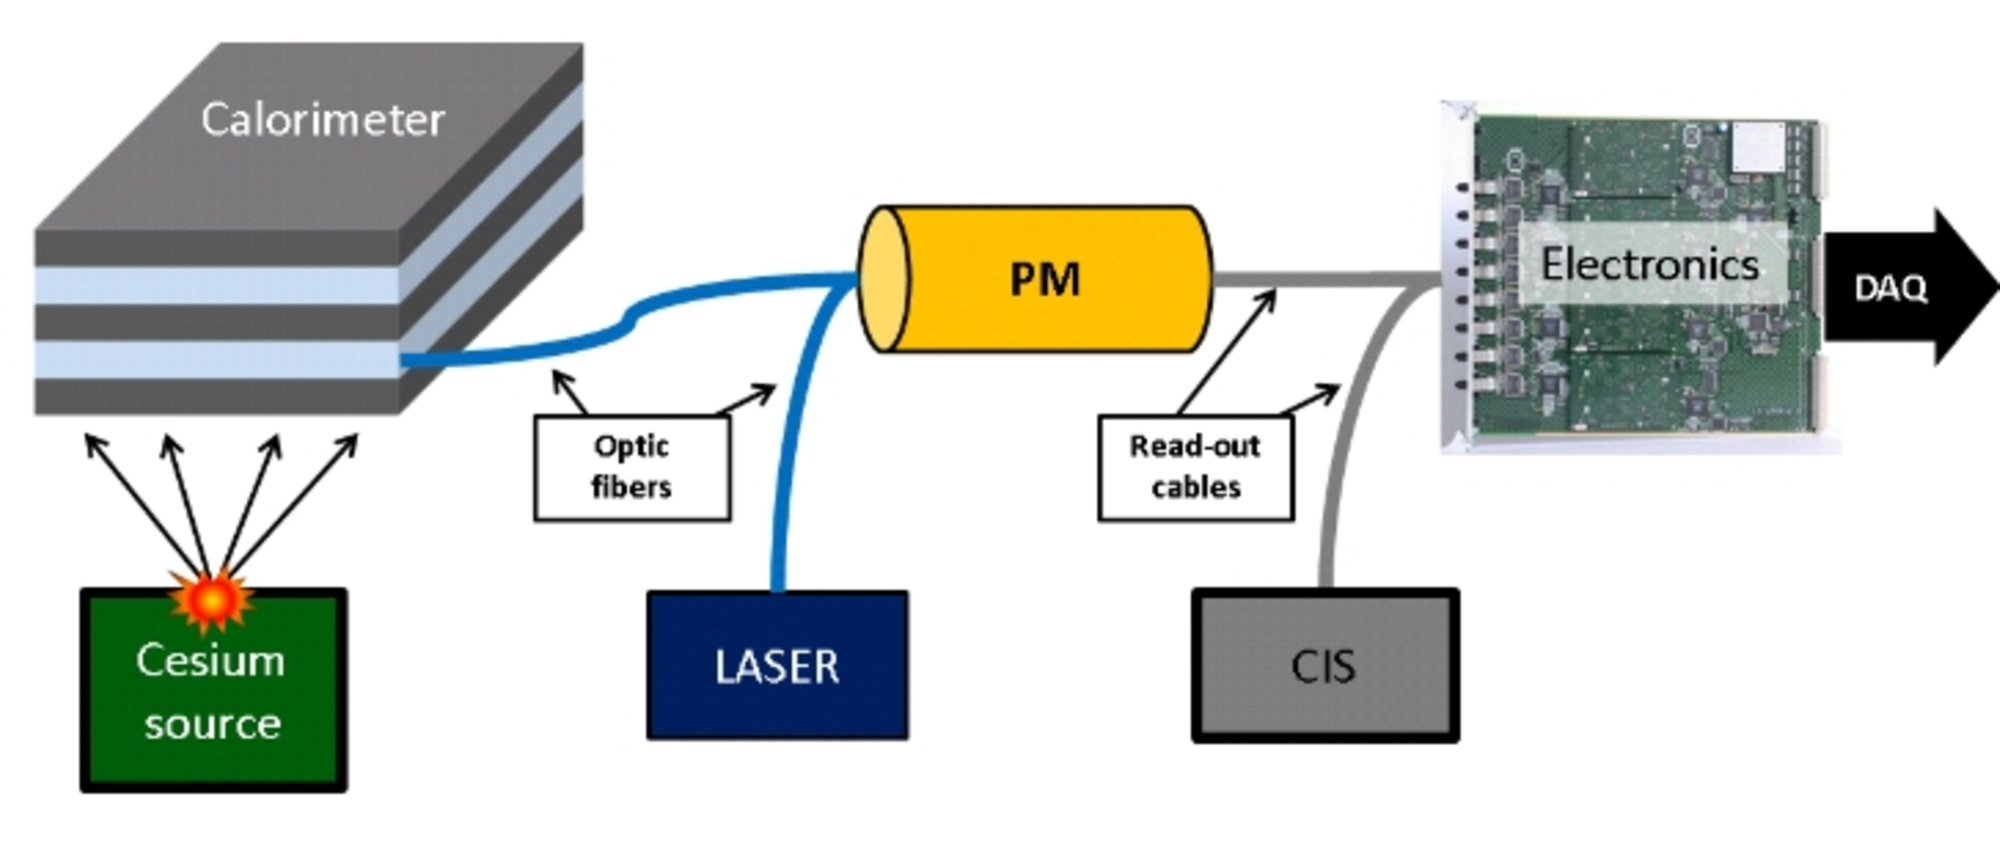
\includegraphics[width=.8\linewidth]{calibration_chain}
    \caption{The ATLAS TileCal calibration chain~\cite{TileCalibChain}.}
    \label{fig:cali_chain}
\end{figure}
%%% Local Variables:
%%% mode: latex
%%% TeX-master: "../search_for_DM_LED_with_ATLAS"
%%% End:
